\documentclass[11pt,aspectratio=169]{beamer}
\usepackage[utf8]{inputenc}
\usepackage{cmap}
\usepackage[T2A]{fontenc}
\usepackage[english,russian]{babel}
\usepackage{graphicx}
\usepackage{booktabs}
\usepackage{amsmath,amssymb}

\graphicspath{{img/}}

\usetheme{Madrid}
\usecolortheme{default}

\title{Определение нижней границы облачности\\ по стереоизображениям}
\author{Устимов И.А.\\[2mm] \small Кафедра математического моделирования и информатики}
\date{Июнь 2026}

\setbeamertemplate{footline}{
  \leavevmode%
  \hbox{%
  \begin{beamercolorbox}[wd=.5\paperwidth,ht=2.25ex,dp=1ex,right]{date in head/foot}%
    \usebeamerfont{date in head/foot}\insertshortdate{}\hspace*{2em}
  \end{beamercolorbox}%
  \begin{beamercolorbox}[wd=.5\paperwidth,ht=2.25ex,dp=1ex,right]{page number in head/foot}%
    \usebeamerfont{page number in head/foot}\insertframenumber{} / \inserttotalframenumber\hspace*{2ex}
  \end{beamercolorbox}}%
}

\begin{document}

%% ========================= TITLE =========================

\begin{frame}
\titlepage
\end{frame}

%% ========================= PLAN =========================

\begin{frame}{План доклада}
\tableofcontents
\end{frame}

%% ================ SECTION: GEOMETRIC MODEL =================

\section{Геометрическая модель}

\begin{frame}{Стереопара: геометрия и формула высоты}
\begin{columns}
\column{0.55\textwidth}
\small
Две камеры с параллельными осями в зенит, база $B$, угол обзора $\phi_0$, облако на высоте $D$. В пиксельных координатах $\xi$:
\[
	D = \frac{B\xi_0}{2\tg(\phi_0/2)|\Delta\xi|},\qquad
	\Delta\xi = \xi_1 - \xi_2
\]

Fisheye ($\phi_0=180^\circ$, $B=45$ м):\;
$D = \frac{\xi_0 \cdot B}{\pi \cdot |\Delta\xi|}$,\;
1 пикс $\approx$ 30 м

\column{0.45\textwidth}
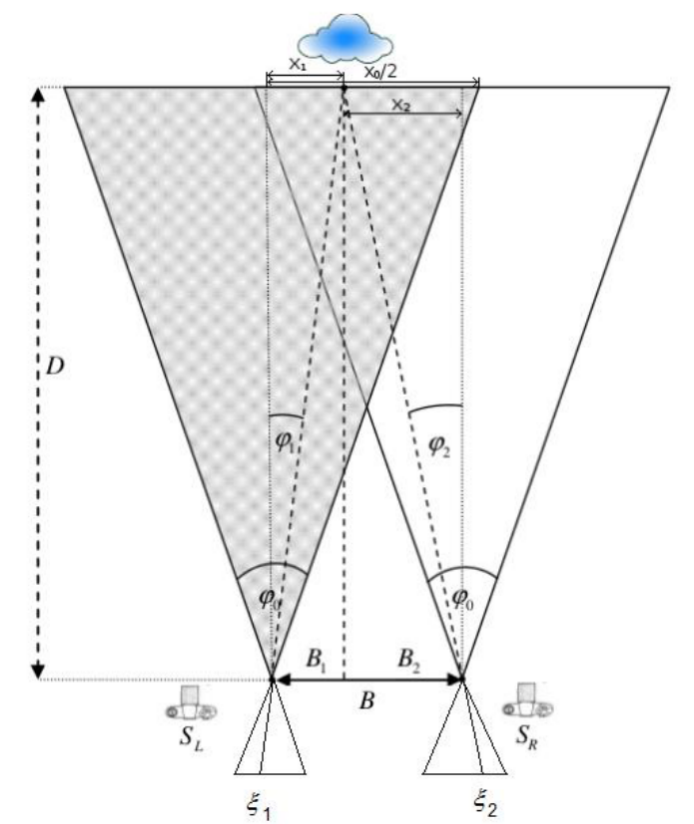
\includegraphics[width=0.9\textwidth]{geom_model}
\end{columns}
\end{frame}

%% ================ SECTION: AFFINE CALIBRATION =================

\section{Калибровка по солнцу}

\begin{frame}{Аффинная калибровка по солнцу}
\begin{columns}
\column{0.55\textwidth}
\begin{block}{Проблема}
	Формула требует \textbf{строго параллельных} оптических осей. В реальности --- всегда есть взаимный поворот и сдвиг камер.
\end{block}

\textbf{Решение:} аффинное преобразование $H$, приводящее снимки к совмещённым осям. Калибровка --- по солнцу (бесконечно удалённый объект; при совмещённых осях его координаты на обоих снимках совпадают).

\vspace{2mm}
\textbf{Порядок обработки:} изображение №1 аффинно преобразуется $\to$ №1$'$; затем ищутся соответствия между №1$'$ и №2.

\column{0.45\textwidth}
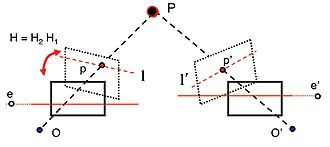
\includegraphics[width=\textwidth]{Rectification}
\end{columns}
\end{frame}

%% ================ SECTION: FEATURE MATCHING =================

\section{Поиск соответствий}

\begin{frame}{LoFTR: плотный нейросетевой мэтчинг}
\begin{columns}
\column{0.47\textwidth}
\textbf{LoFTR} (Local Feature TRansformer):
\begin{itemize}
	\item \textbf{Detector-free} --- не требует выделения ключевых точек
	\item ViT-архитектура: патчи $\to$ эмбеддинги $\to$ attention по всему изображению
	\item Плотные предсказания на малом расстоянии
	\item Предобучена на больших наборах данных
\end{itemize}

\column{0.53\textwidth}
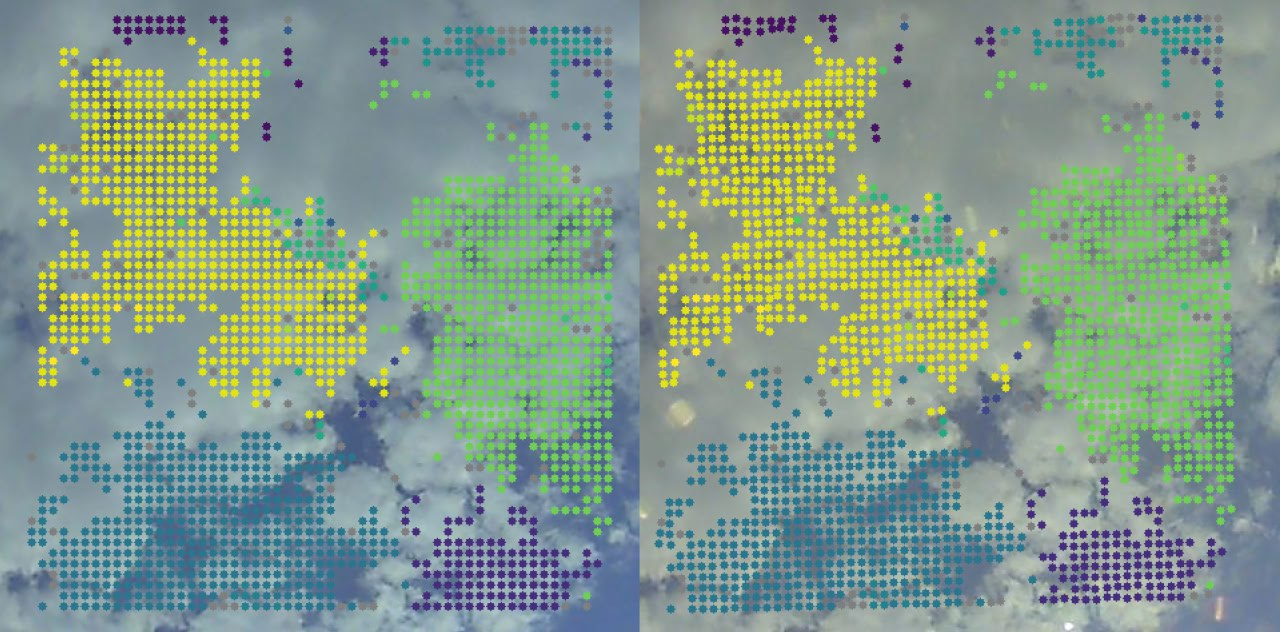
\includegraphics[width=\textwidth]{loftr_clouds}
\end{columns}

\vspace{2mm}
{\small Зелёные линии --- найденные LOFTR соответствия. Смещение $\Delta\vec r = (x'_1 - x_2,\; y'_1 - y_2)$; для формулы высоты нужна только $x$-компонента $\Delta\xi$.}
\end{frame}

%% ================ SECTION: CLUSTERING =================

\section{Кластеризация}

\begin{frame}{HDBSCAN: группировка по смещениям}
\begin{columns}
\column{0.50\textwidth}
\textbf{Проблема:} LoFTR даёт сотни соответствий + ложные мэтчи. Нужно выделить основные облачные слои.

\vspace{2mm}
\textbf{HDBSCAN} --- иерархическая плотностная кластеризация в пространстве векторов смещений:
\begin{itemize}
	\item Не требует числа кластеров априори
	\item Автоматически определяет шум
	\item Каждый кластер $\leftrightarrow$ свой слой облачности
\end{itemize}

\column{0.50\textwidth}
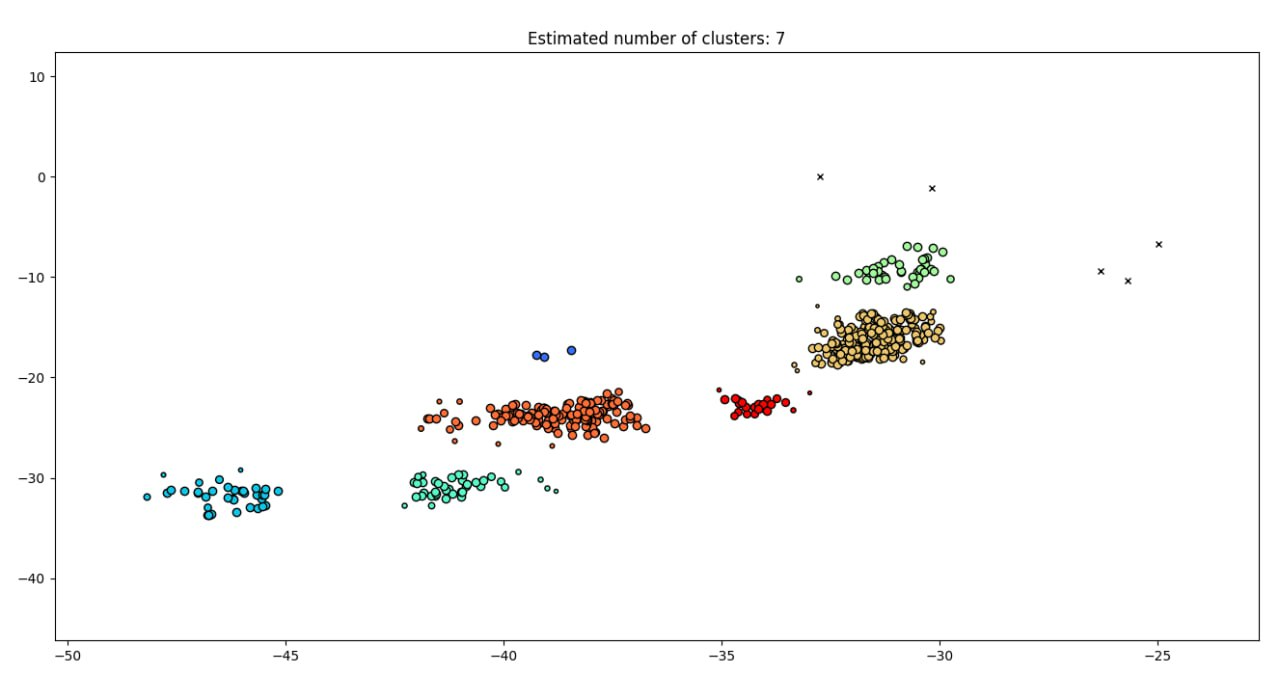
\includegraphics[width=0.85\textwidth]{cluster}\\[2mm]
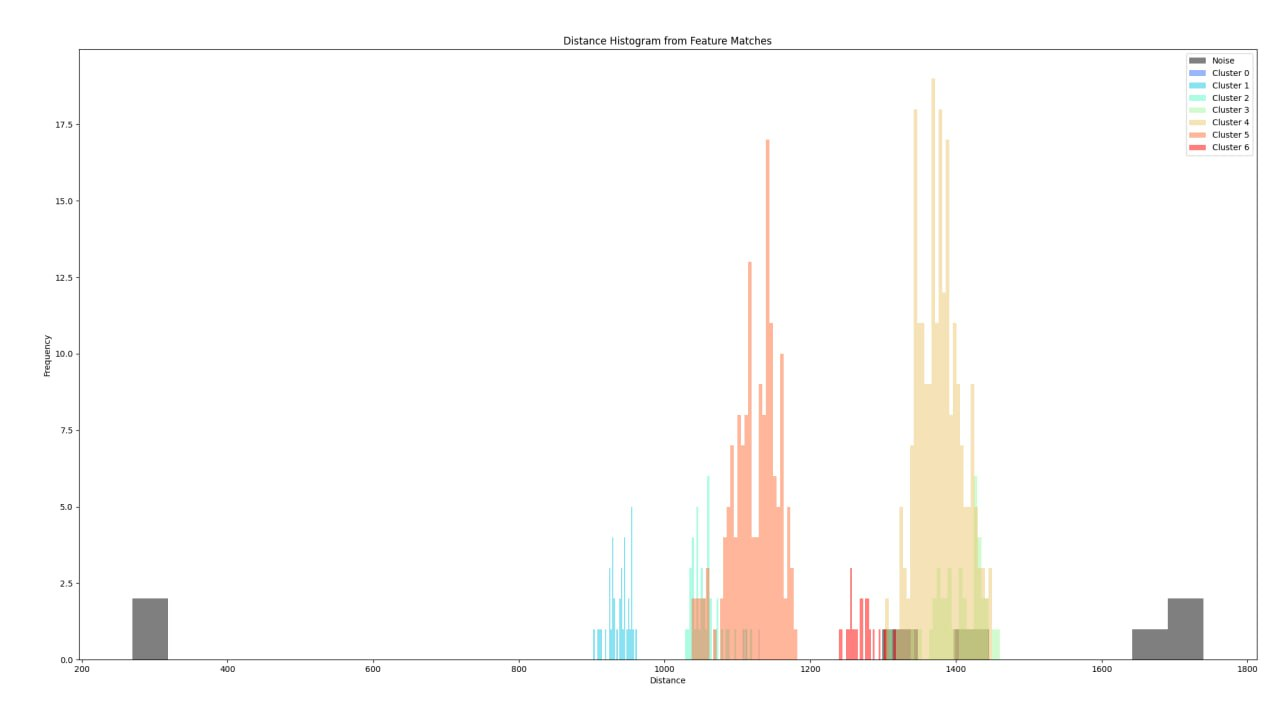
\includegraphics[width=0.85\textwidth]{height_dist}
\end{columns}
\end{frame}

%% ================ SECTION: LIMITATIONS =================

\section{Проблемы покадрового подхода}

\begin{frame}{Что не так с независимым анализом кадров?}
\begin{alertblock}{Ограничения}
\begin{itemize}
	\item Каждый кадр обрабатывается \textbf{независимо} --- нет памяти
	\item \textbf{Скачки высоты:} до 500 м за 10 с ($\sim$50 м/с --- нереалистично)
	\item \textbf{Низкая автокорреляция:} $r_\text{auto} \approx 0.11$ (5 ч) --- ряд физически несогласован
	\item Пространственная неконсистентность: точки с одинаковым смещением могут быть из разных участков неба $\to$ <<паразитные>> кластеры
\end{itemize}
\end{alertblock}

\vspace{2mm}
\textbf{Необходимы:}
\begin{enumerate}
	\item Пространственная фильтрация кластеров
	\item Временной фильтр
\end{enumerate}
\end{frame}

%% ================ SECTION: SPATIAL FILTER =================

\section{Пространственная фильтрация}

\begin{frame}{Пространственная фильтрация кластеров}
HDBSCAN кластеризует по смещению, но \textbf{не проверяет} физическую связность точек в плоскости изображения.

\vspace{2mm}
\textbf{Три стадии проверки:}
\begin{enumerate}
	\item \textbf{DBSCAN-субкластеризация} ($\varepsilon = 30$ px) --- отсев пространственно разрозненных групп
	\item \textbf{Проверка плотности} (ConvexHull, $\rho_\text{min} = 0.002$ pts/px$^2$) --- отсев <<пылевых>> кластеров
	\item \textbf{Согласованность смещений} ($K=5$ соседей) --- <<близкие в изображении $\Rightarrow$ близкие по смещению>>
\end{enumerate}

\vspace{2mm}
\textbf{Результат:} отсеивается 15--25\% кластеров, повышается чистота входа временного фильтра.
\end{frame}

%% ================ SECTION: KALMAN FILTER =================

\section{Временной фильтр Калмана}

\begin{frame}{Постановка задачи временной фильтрации}
Дана последовательность зашумлённых оценок высоты $\{z_t\}_{t=1}^T$ по каждому кадру. Соседние оценки содержат выбросы (скачки до 500 м за 10 с). Требуется получить сглаженную траекторию, согласованную с физикой. Модель эволюции --- равномерное движение:
\[
	h_{t+1} = h_t + \dot{h}_t \Delta t, \qquad \dot{h}_{t+1} = \dot{h}_t
\]
Задача: восстановить скрытое состояние $\mathbf{x}_t = [h_t, \dot{h}_t]^\top$ при неизвестной дисперсии шума и выбросах.
\end{frame}

\begin{frame}{Фильтр Калмана: модель и результаты}
\textbf{Модель процесса:}
\[
	\mathbf{x} = [h, \dot{h}]^\top, \quad
	\mathbf{F} = \begin{pmatrix} 1 & \Delta t \\ 0 & 1 \end{pmatrix}
\]

\textbf{Отличительная особенность:} адаптивная настройка шума измерений $R$ по величине невязки $|z - \hat{x}^-|$ --- при малой невязке фильтр доверяет измерению, при большой (выброс) --- предсказанию.

\vspace{2mm}
\begin{table}
\centering
\begin{tabular}{lccc}
\toprule
Метрика & Исходные & После фильтра & Улучшение \\
\midrule
Средний перепад $|\Delta h|$ (10 с) & 515 м & 120 м & \textbf{в 4.3 раза} \\
Автокорреляция (5 ч) & 0.11 & 0.90 & \textbf{в 8.0 раз} \\
Средняя $r$ (30-мин окна) & 0.55 & 0.61 & +11\% \\
Доля окон с $r > 0.5$ & 61\% (11/18) & 72\% (13/18) & --- \\
Максимальная $r$ в окне & 0.88 & 0.94 & --- \\
\bottomrule
\end{tabular}
\end{table}
\end{frame}

\begin{frame}{Сшитый временной ряд: 30-минутные окна}
\begin{center}
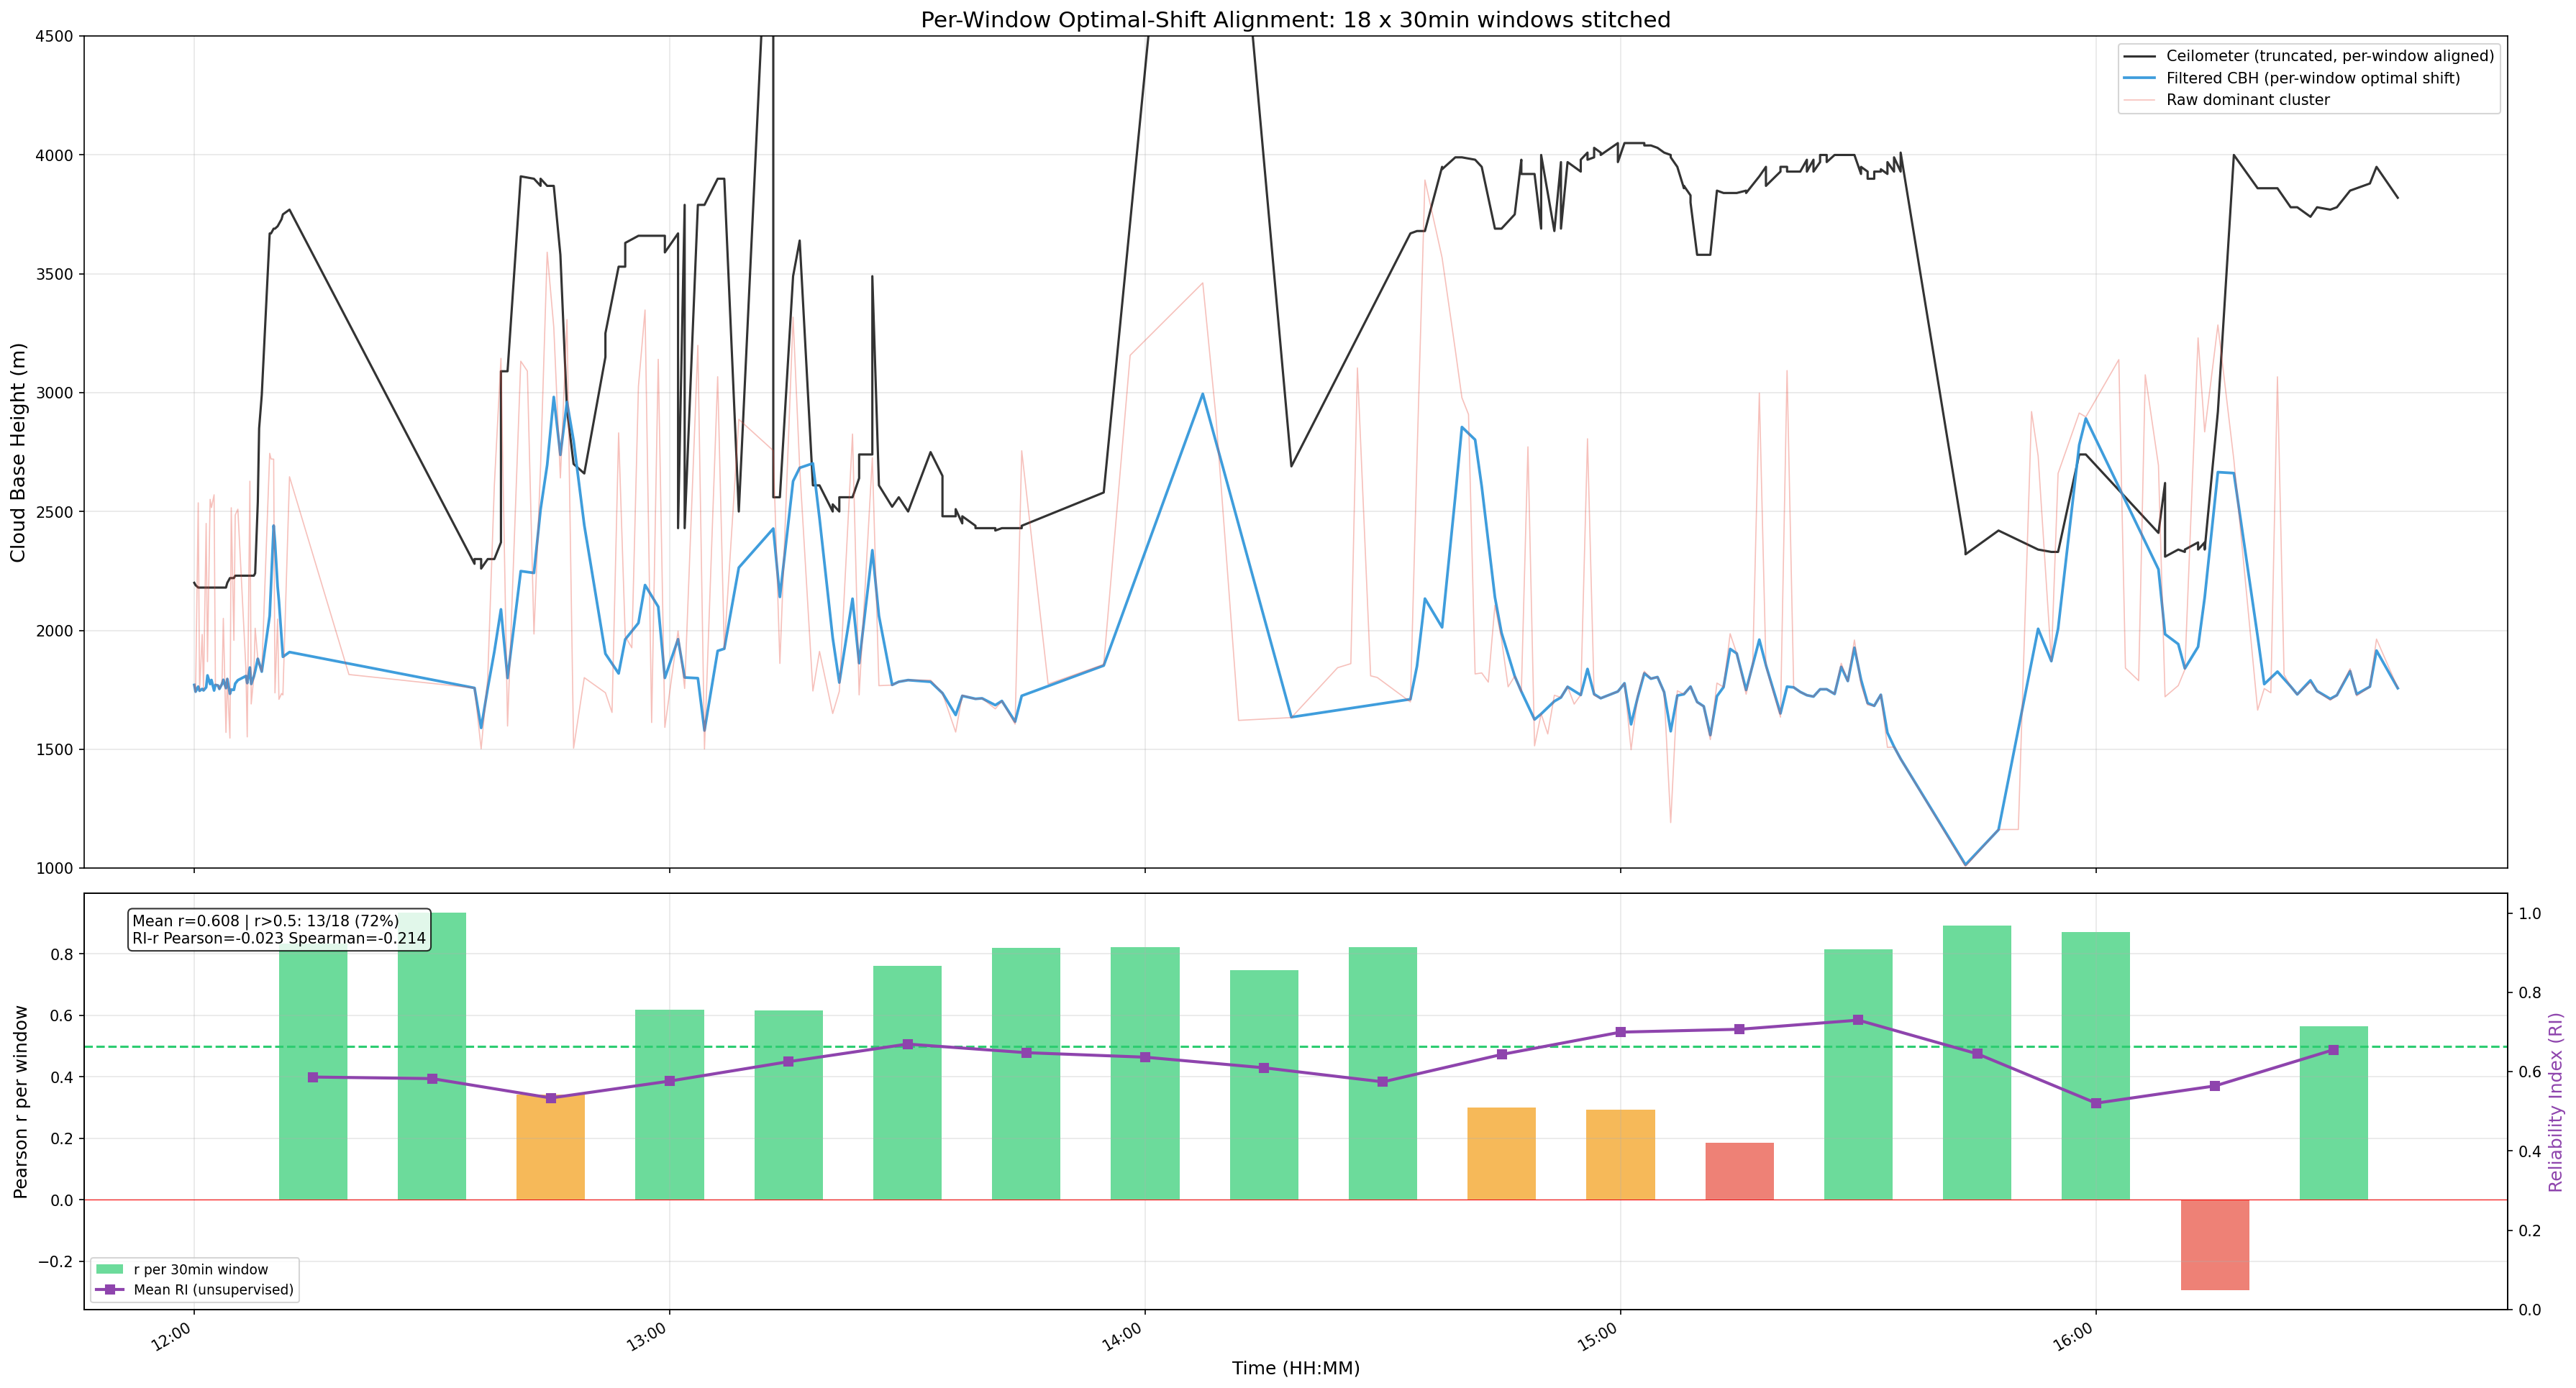
\includegraphics[width=0.85\textwidth,height=0.78\textheight,keepaspectratio]{01_stitched_windows}
\end{center}
\end{frame}

\begin{frame}{Примеры кадров}
\begin{columns}
\column{0.50\textwidth}
\centering
\textbf{12:00, $r = 0.74$}\\[1mm]
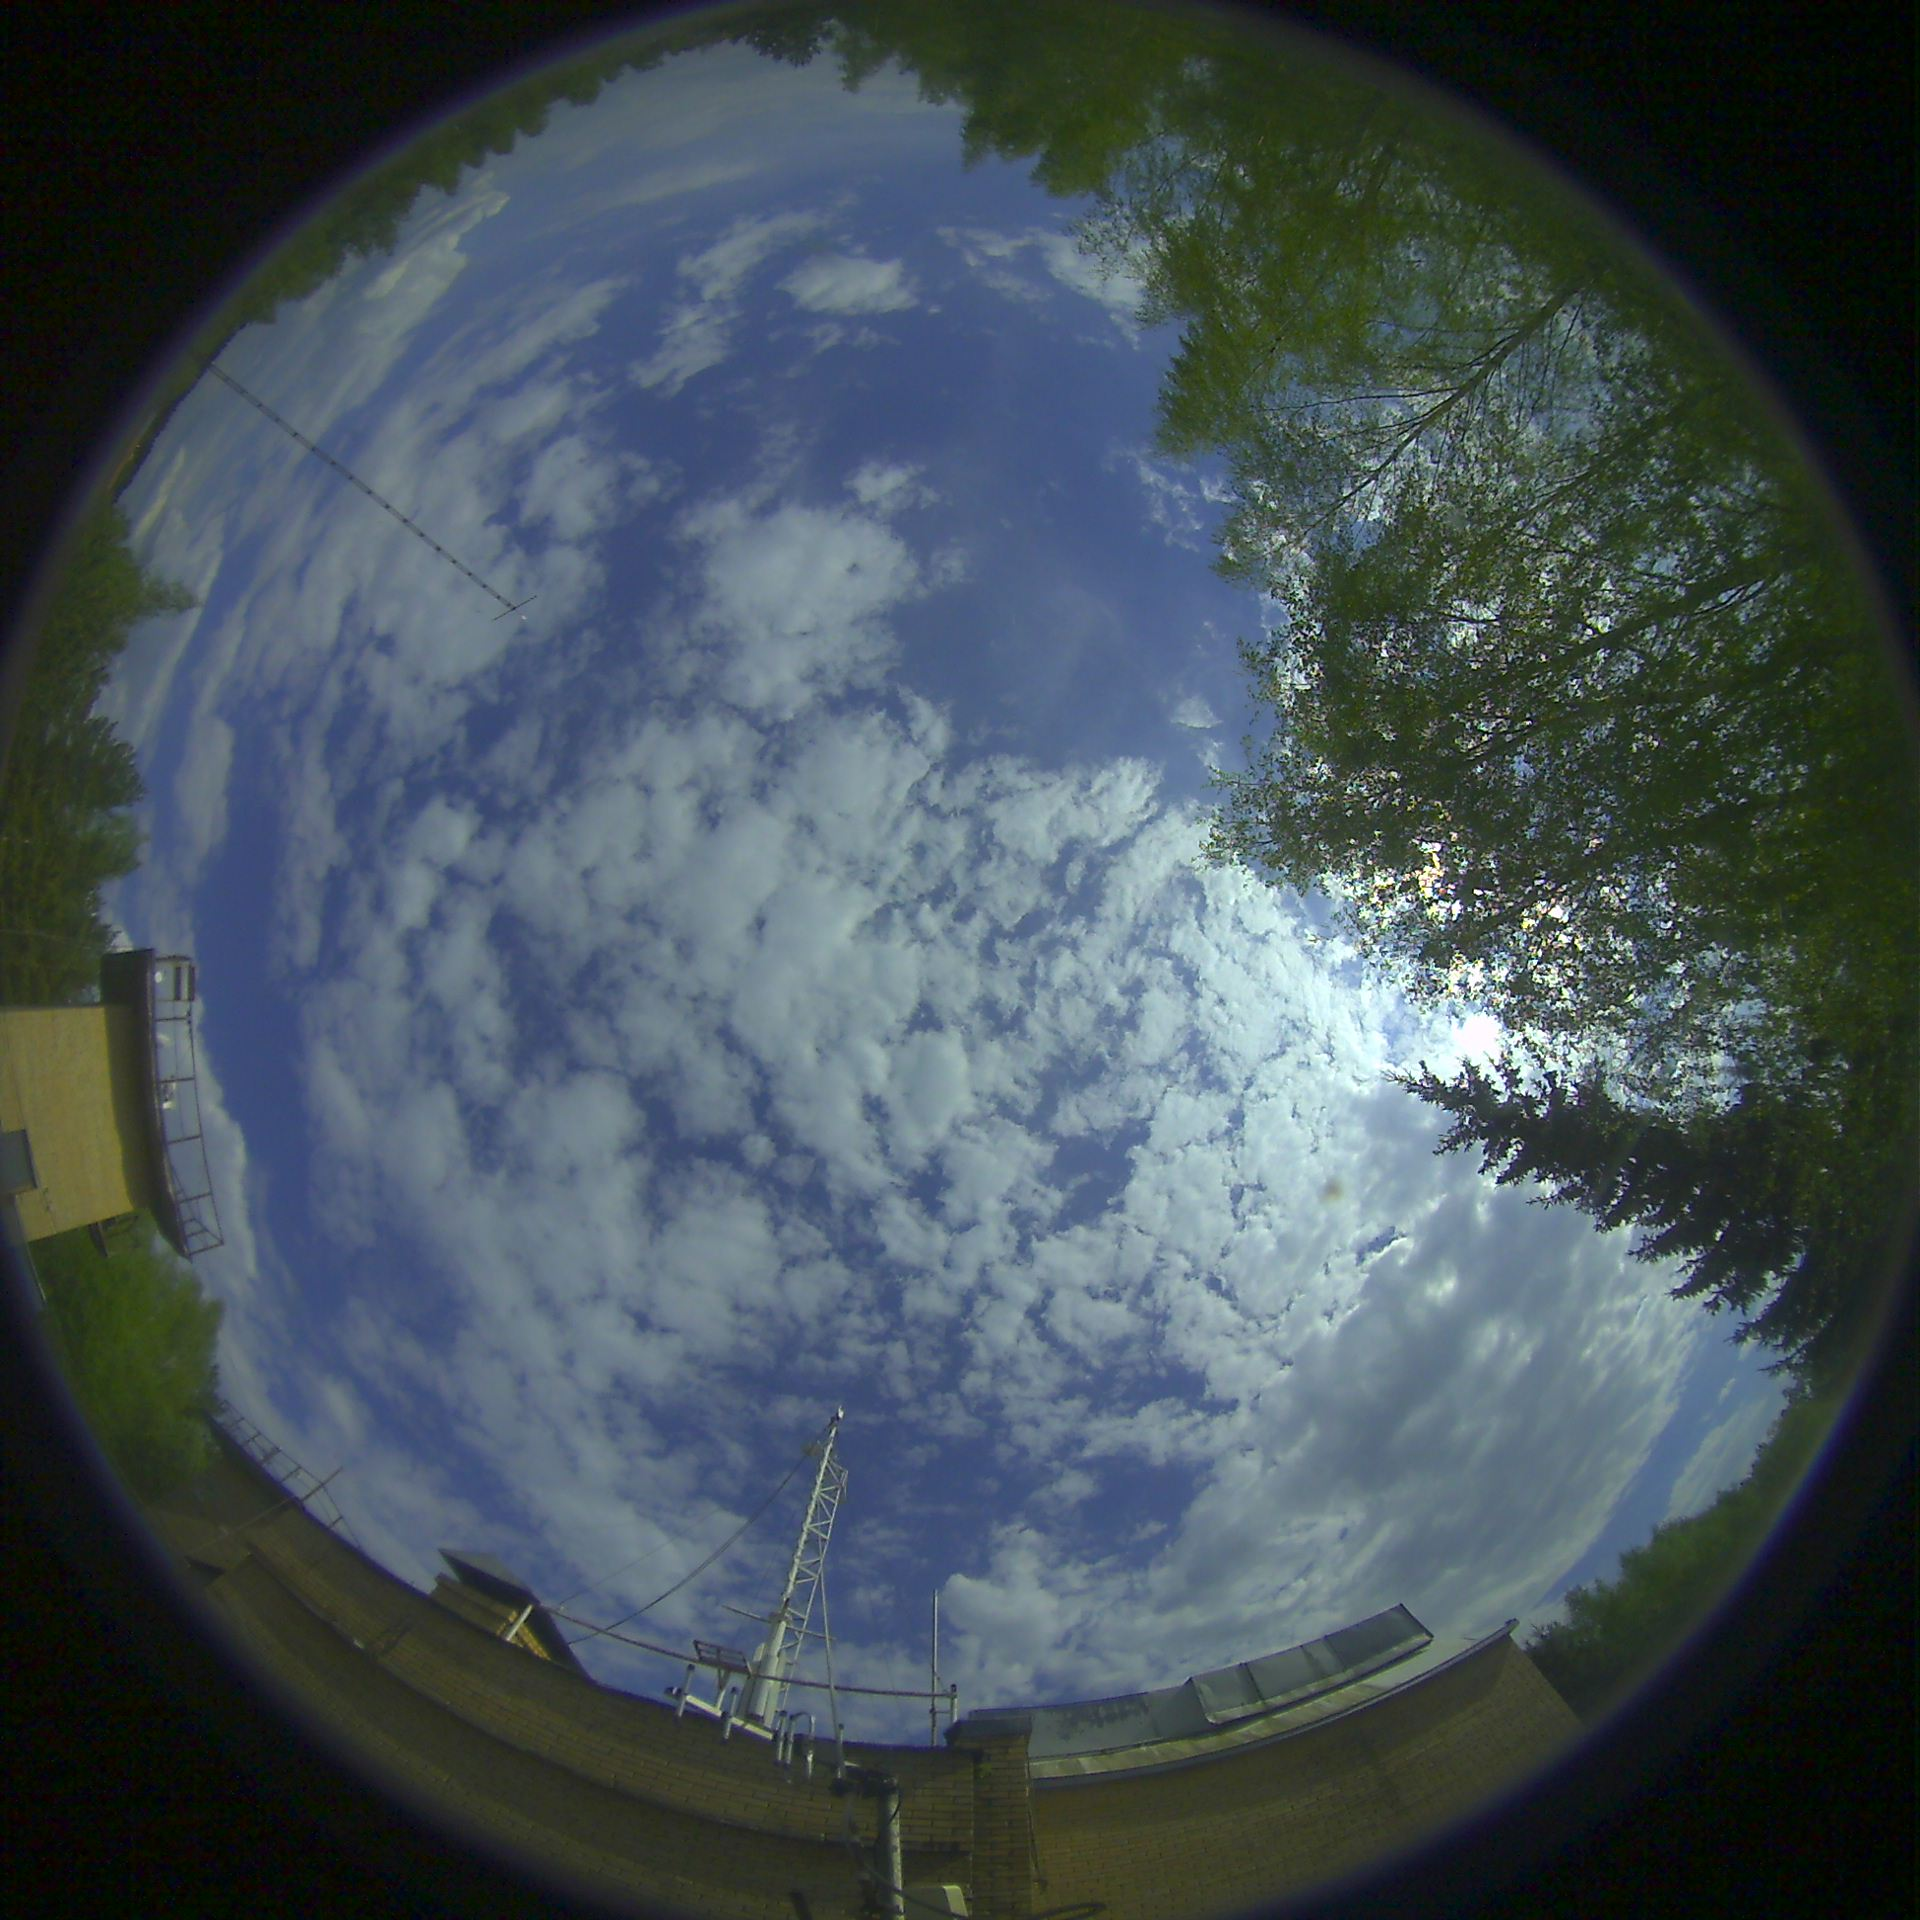
\includegraphics[width=0.95\textwidth,height=0.42\textheight,keepaspectratio]{img-2025-05-23T12-00-01devID1}
\vspace{1mm}
{\small Однородная облачность; однозначное смещение.}

\column{0.50\textwidth}
\centering
\textbf{16:30, $r = 0.66$}\\[1mm]
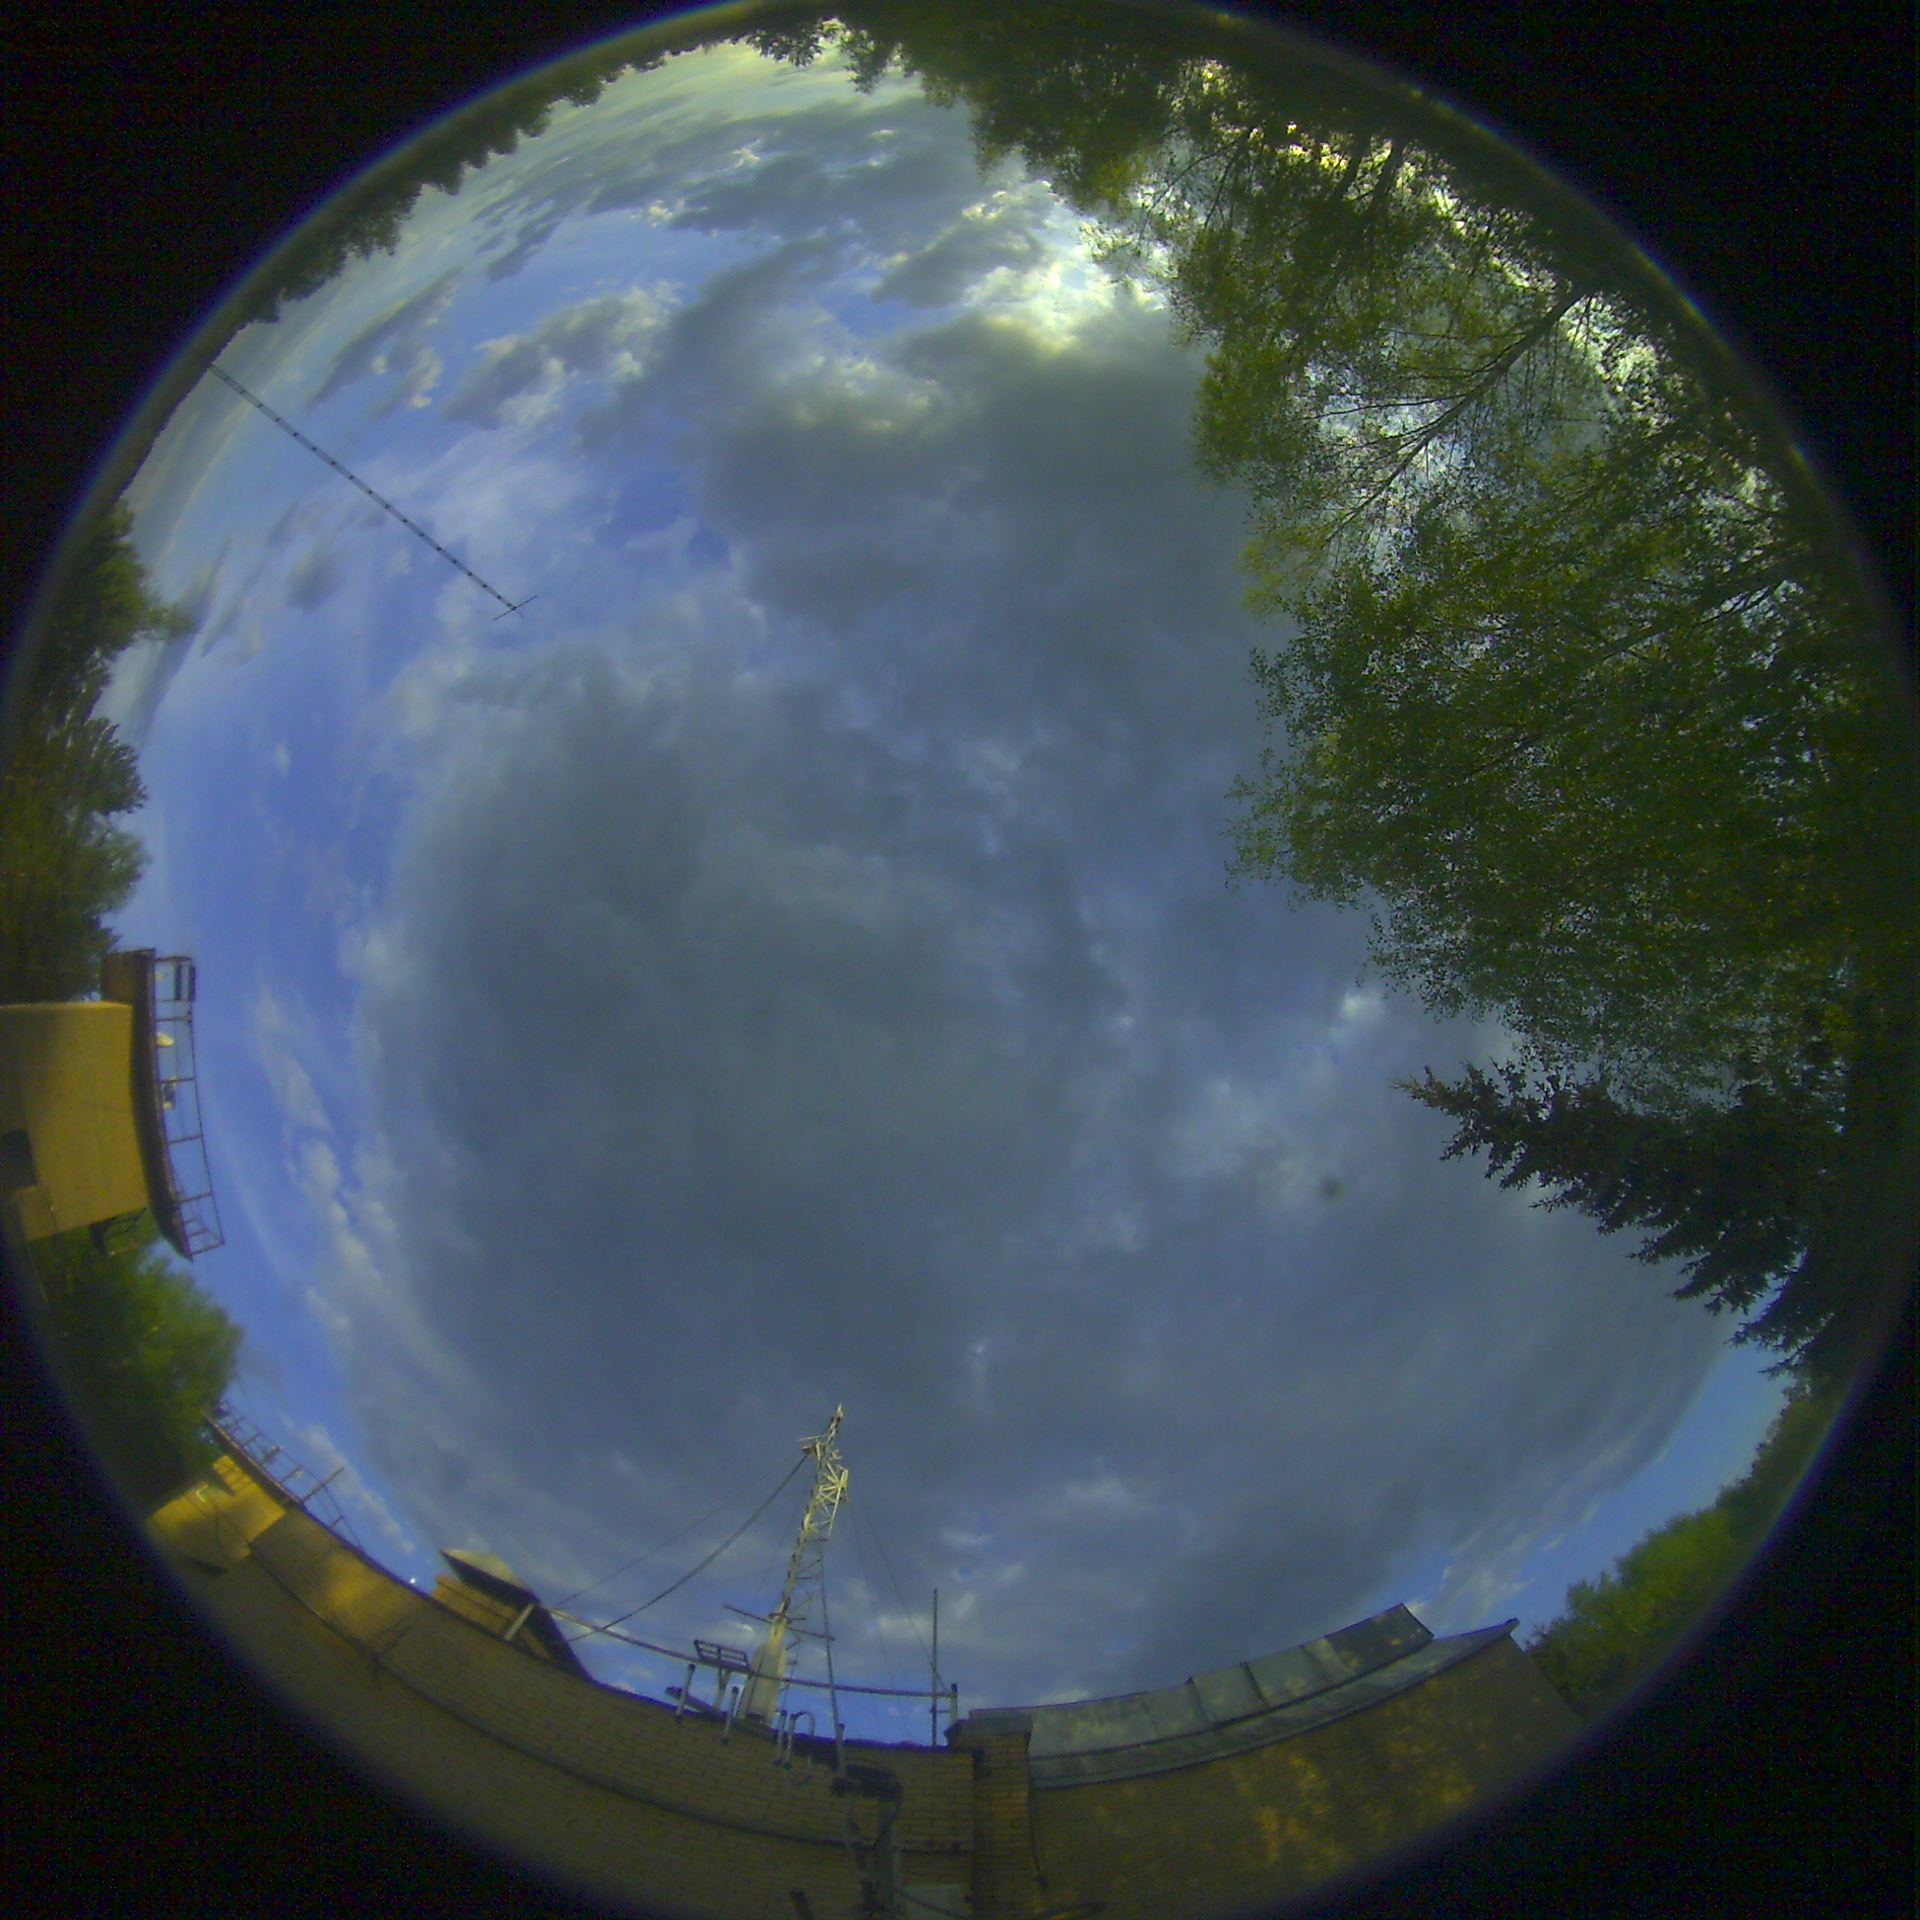
\includegraphics[width=0.95\textwidth,height=0.42\textheight,keepaspectratio]{img-2025-05-23T16-30-04devID1}
\vspace{1mm}
{\small Многослойная облачность; несколько слоёв с разной скоростью.}
\end{columns}
\end{frame}

%% ================ SECTION: DYNAMIC SHIFT =================

\section{Анализ временных сдвигов}

\begin{frame}{Динамический временной сдвиг}
\begin{columns}
\column{0.50\textwidth}
\small
\textbf{Проблема:} ветер сносит облака между моментами измерений алгоритма и высотомера --- возникает переменный временной лаг, разрушающий корреляцию.

\vspace{2mm}
\textbf{Метод:} разбиение временного ряда на скользящие окна, в каждом окне подбирается оптимальный глобальный сдвиг $\Delta t$, максимизирующий $r$ Пирсона:
\[
\Delta t^* = \arg\max_{\Delta t}\;\bigl|\mathrm{corr}\bigl(H_{\text{ceilo}}(t),\; H_{\text{algo}}(t+\Delta t)\bigr)\bigr|
\]

\vspace{2mm}
Физический смысл $\Delta t$ --- прокси угла сноса ветра: $\Delta t = \frac{D}{V} \cos\theta$.

\column{0.50\textwidth}
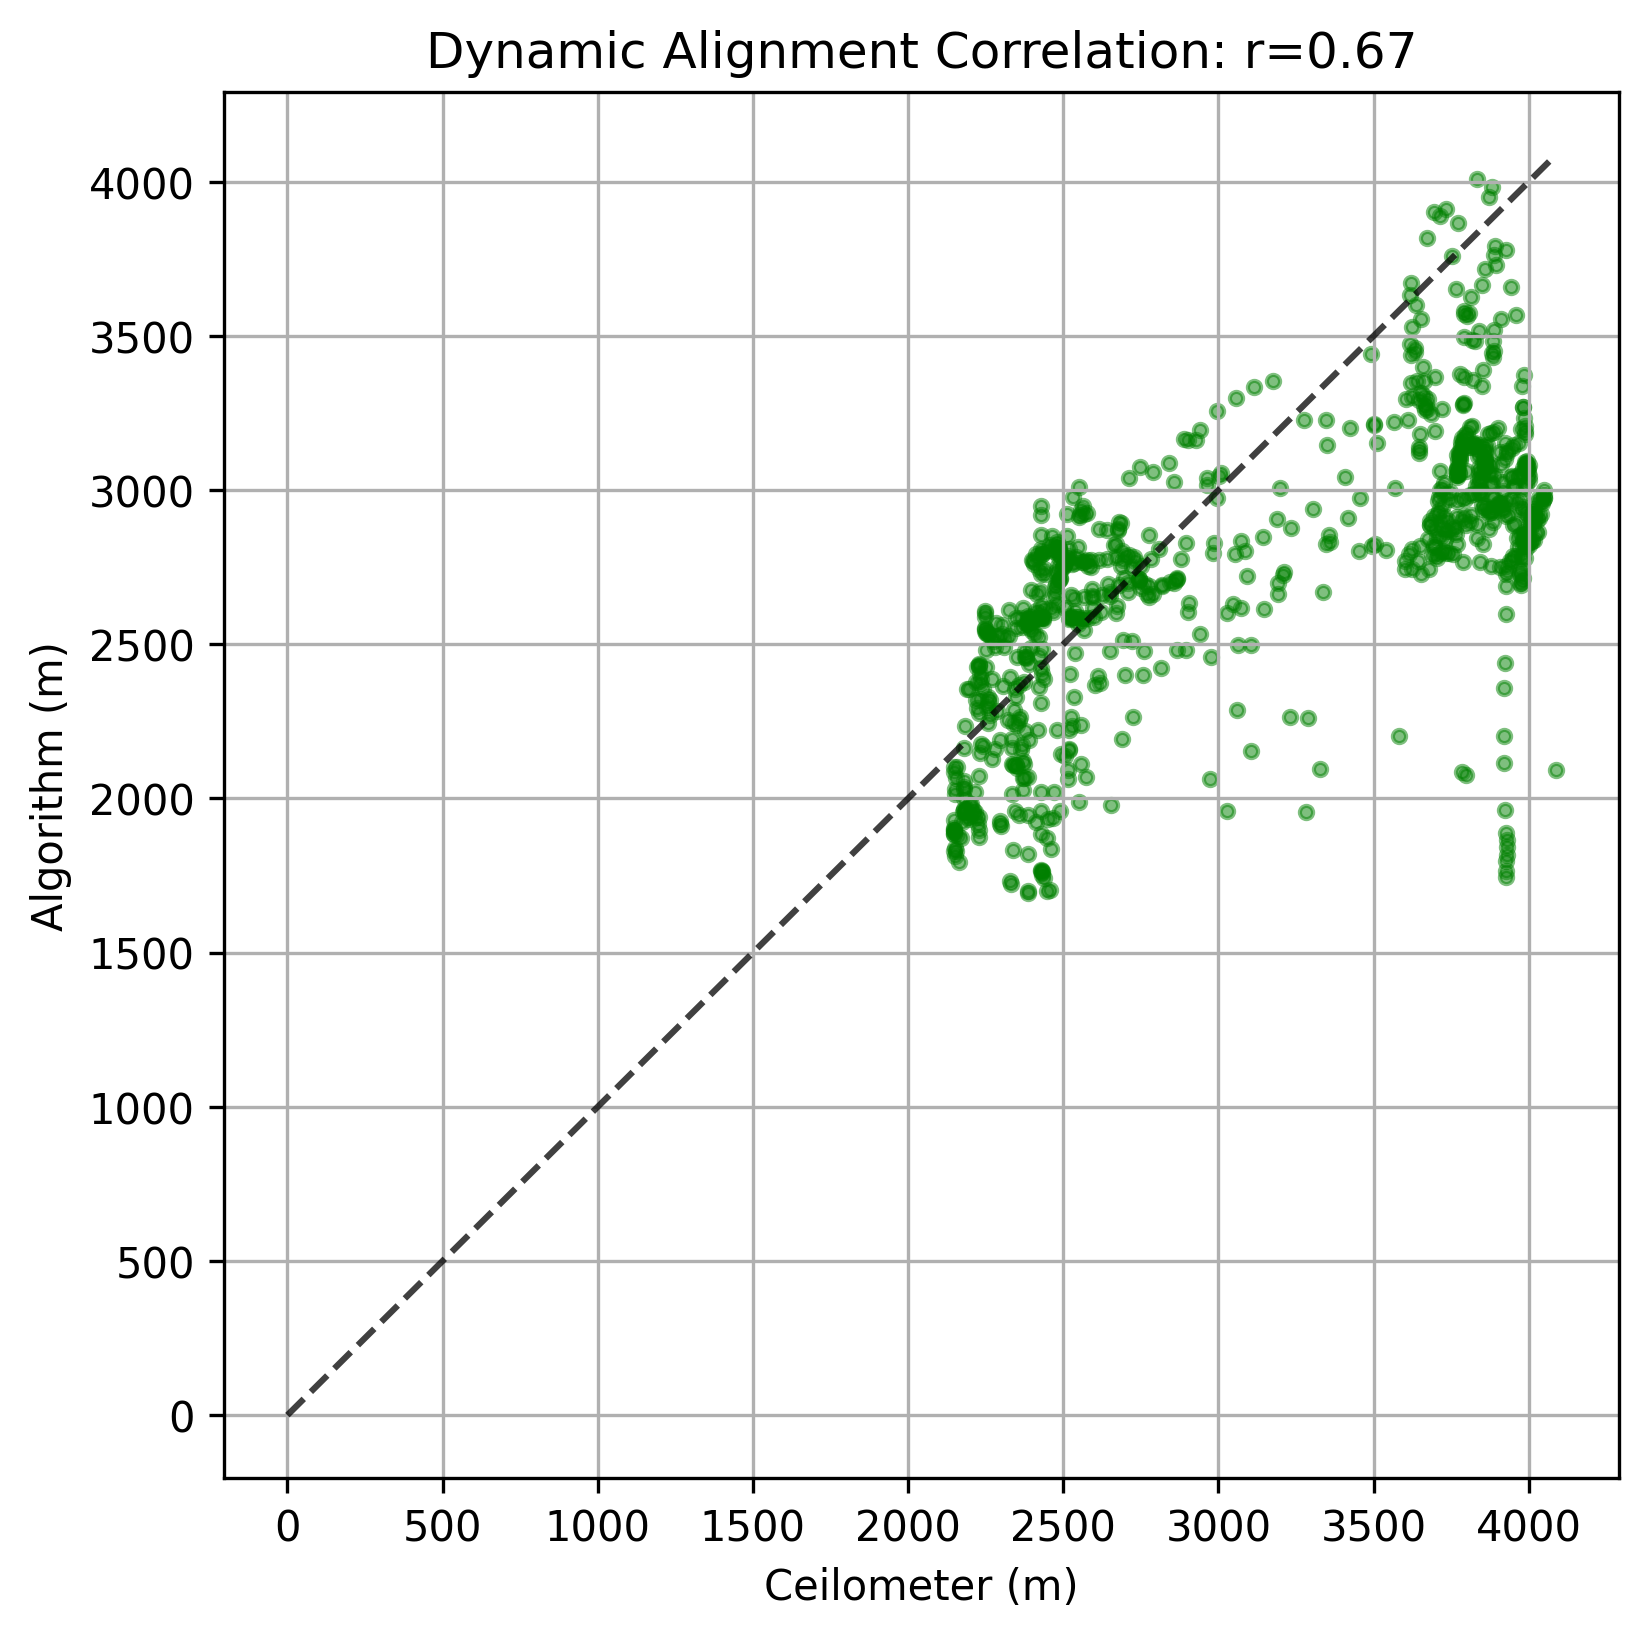
\includegraphics[width=\textwidth]{correlation_dynamic}
\end{columns}
\end{frame}

\begin{frame}{Профиль динамического сдвига}
\begin{columns}
\column{0.50\textwidth}
\small
Скользящее окно 5 минут, поиск $\pm 300$ с. Сдвиг $\Delta t$ меняется от $-240$ до $+170$ с в течение дня --- отражает смену направления и силы ветра.

\vspace{2mm}
\textbf{Результат:} после динамической компенсации сдвига:
\begin{itemize}
  \item Средняя $r$ (30-мин окна): $0{,}61$
  \item 72\% окон с $r > 0{,}5$
  \item $\max r = 0{,}94$
\end{itemize}

\column{0.50\textwidth}
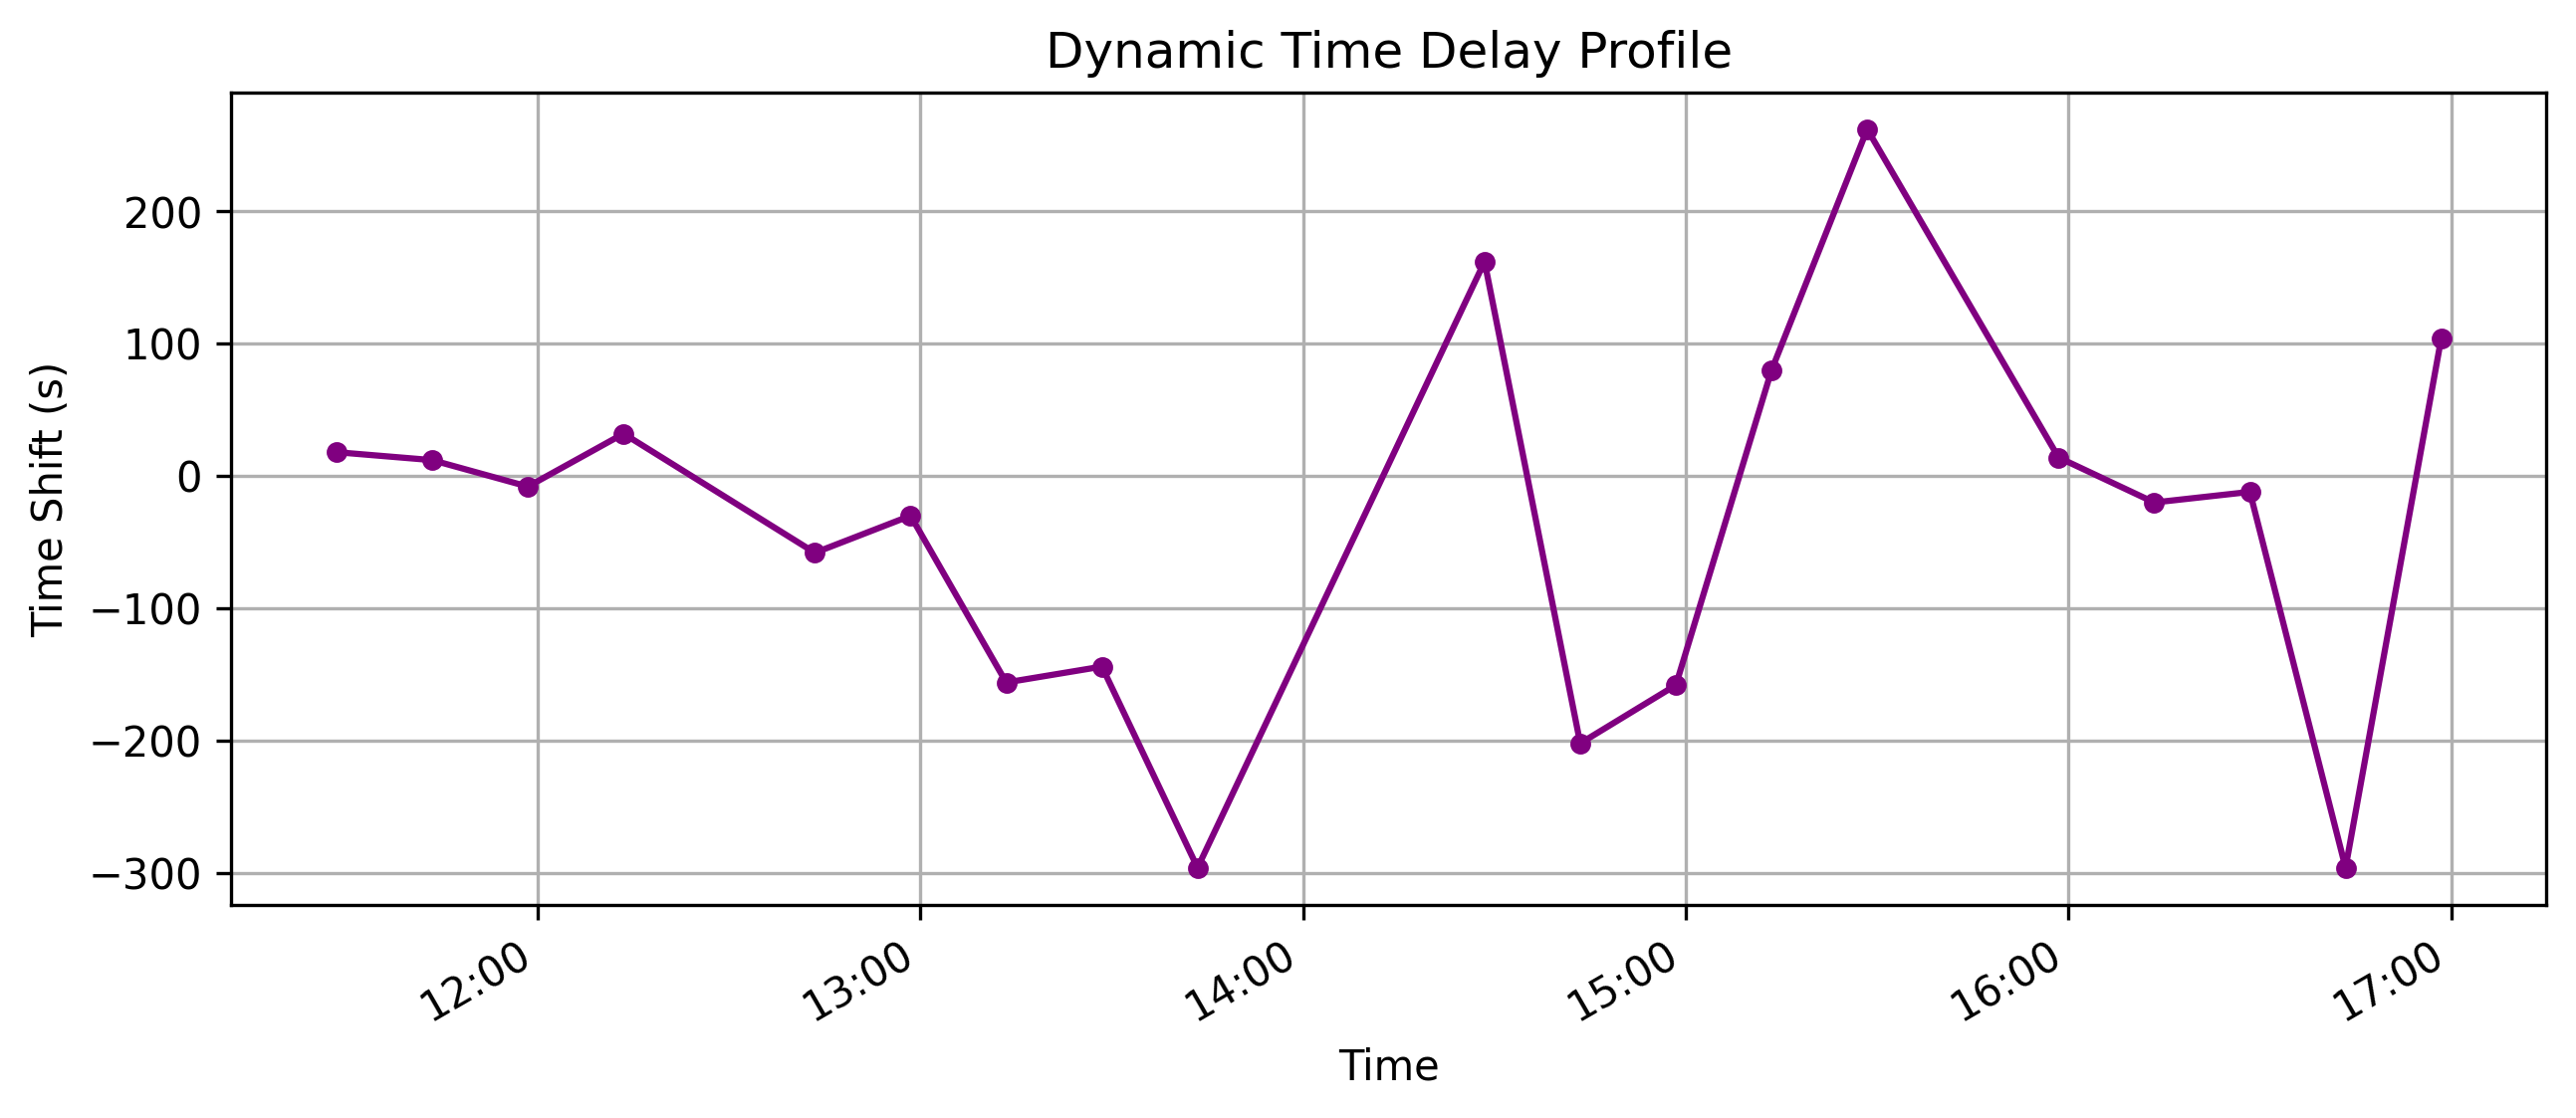
\includegraphics[width=\textwidth]{dynamic_shift_profile}
\end{columns}
\end{frame}

%% ================ SECTION: CEILOMETER BIAS =================

\section{Смещение высотомера}

\begin{frame}{Эталонный прибор: высотомер ДОЛ-2}
\begin{columns}
\column{0.50\textwidth}
\textbf{ДОЛ-2} --- лазерный облакомер (датчик высоты облаков):
\begin{itemize}
	\item Источник: полупроводниковый импульсный лазер
	\item Принцип: измерение обратно рассеянного зондирующего импульса
	\item Диапазон: 10--3000 м
	\item Погрешность: $\pm 10$ м (до 100 м), $\pm(5 + 0{,}05H)$ м (100--3000 м)
	\item Частота: 1 измерение / 15 с
\end{itemize}

\column{0.50\textwidth}
\textbf{Систематическое завышение:}
\begin{itemize}
	\item Отражённый сигнал достигает порога детекции лишь на некоторой глубине внутри облака
	\item Измеряется \textbf{оптическая}, а не геометрическая граница
	\item Стереосистема измеряет \textbf{геометрическую} границу --- по рассеянному солнечному свету
\end{itemize}

\vspace{2mm}
$\Rightarrow$ \textbf{Стереометод и высотомер измеряют принципиально разные величины.} Этим объясняется систематическое вертикальное смещение между рядами.
\end{columns}
\end{frame}

%% ================ SECTION: CONCLUSIONS =================

\section{Заключение}

\begin{frame}{Выводы}
\begin{enumerate}
	\item \textbf{Стереометод с fisheye-камерами} даёт оценку геометрической НГО, принципиально отличную от оптической оценки высотомера
	\item \textbf{Корреляция с высотомером} --- в 72\% (13 из 18) 30-минутных окон $r > 0.5$; в остальных окнах --- многослойная облачность и смена направления ветра
	\item \textbf{Фильтр Калмана} снижает перепады высоты в 4.3 раза, повышает автокорреляцию с 0.11 до 0.90 --- ряд становится физически согласованным
	\item \textbf{Пространственная фильтрация} отсеивает 15--25\% нефизичных кластеров до подачи в трекер
	\item \textbf{Ограничения:} калибровка нестабильна во времени (температурные деформации); при сплошной облачности без текстурных особенностей метод не работает
\end{enumerate}
\end{frame}

\begin{frame}{Спасибо за внимание}
\begin{center}
\Large
Вопросы?
\end{center}
\end{frame}

\end{document}
